%% V0.2
%% by Luis Felipe Wolf Batista, luisfelipewb@gmail.com
%% This is a template for Udacity projects using IEEEtran.cls


\documentclass[10pt,journal,compsoc]{IEEEtran}

\usepackage[pdftex]{graphicx}    
\graphicspath{{img/}}
\usepackage{subfig}
\usepackage{cite}
\hyphenation{op-tical net-works semi-conduc-tor}


\begin{document}

\title{Robotic Inference}

\author{Luis F. W. Batista}

\markboth{Inference project, Robotic Nanodegree, Udacity}%
{}
\IEEEtitleabstractindextext{%

\begin{abstract}
Perception using Neural Networks is widely used in modern robotic applications. This report presents the results obtained from two popular Neural Networks used to perform image classification. The results are presented considering the constraints imposed by embedded systems such as limited energy supply and maximum inference time. The conclusion is that a simpler model is often the best choice if it can achieve the desired accuracy. The outcome of this investigation will be used for a home robot that can autonomously locate objects around the house. 

\end{abstract}

% Note that keywords are not normally used for peerreview papers.
\begin{IEEEkeywords}
Robot, IEEEtran, Udacity, \LaTeX, deep learning.
\end{IEEEkeywords}}

\maketitle
\IEEEdisplaynontitleabstractindextext
\IEEEpeerreviewmaketitle
\section{Introduction}
\label{sec:introduction}

\IEEEPARstart{A}{utonomous} robots can be very useful for a broad range of applications including find and fetch objects. This use can be very beneficial especially for elder care, where locomotion may require a lot of effort. For instance, a robot could autonomously locate and bring a specific medicine even if the person does not know where it is. 

Approaches to accomplish this mission have been made using RFID technology \cite{inproceedings} but requires that each object is previously identified with a physical tag. A more flexible option is to use modern Machine Learning techniques combining camera sensors and Neural Networks to perform object recognition. 

The drawback is that such applications demand large hardware resources. If latency and connectivity is not a concern, image recognition can be implemented in the cloud. Unfortunately, it is usually not possible as many mission-critical applications demand a very fast response time and have unreliable connectivity. It is also common to run on batteries and require efficient use of the available power.

Recent studies show that energy constraint is an upper bound on maximum achievable accuracy and model complexity \cite{Canziani2017AnAO}. In other words, to preserve battery on a robotic application, one should find the model with lower complexity that can achieve the desired accuracy given a maximum inference time. 

With the intention of exploring the performance of machine learning in robotic applications with limited hardware resources, this report presents a comparison of two prototype inference models using two widely known architectures: AlexNet \cite{NIPS2012_4824} and GoogLeNet \cite{GLN43022}. The desire is to establish the foundation that will be used later in a project to autonomously recognize common objects inside the house.

\section{Background / Formulation}

This project is part of the Robotics Software Engineer Nanodegree from Udacity. Two datasets were used to train two types of deep neural network models used for inferencing. The first dataset was provided in the course material and was used for learning purposes. The second dataset was collected from random objects that can be found at a house.

The models were trained in a virtual environment using the NVIDIA DIGITS workflow. Initially, the same hyperparameters were used for easy comparison. To improve the results the parameters were adjusted and the final values used are shown in Table \ref{tab:hyperparameters}.

\begin{table}[]
\centering
\begin{tabular}{l|c|c|c|c|}
\cline{2-5}
                                                & \multicolumn{2}{c|}{\textbf{Supplied Dataset}} & \multicolumn{2}{c|}{\textbf{Collected Dataset}} \\ \cline{2-5} 
                                                & AlexNet               & GoogLeNet              & AlexNet               & GoogLeNet               \\ \hline
\multicolumn{1}{|l|}{\textbf{Number of epochs}} & 6                     & 6                      & 20                    & 20                      \\ \hline
\multicolumn{1}{|l|}{Initial learning rate}     & 0.01                  & 0.01                   & 0.01                  & 0.01                    \\ \hline
\multicolumn{1}{|l|}{\textbf{Decrease Fator}}   & 0.1                   & 0.1                    & 0.8                   & 0.1                     \\ \hline
\multicolumn{1}{|l|}{Number of Steps}           & 3                     & 3                      & 10                    & 3                       \\ \hline
\end{tabular}
\caption{Hyperparameters}
\label{tab:hyperparameters}
\end{table}

Finally, the inference time of each model trained with the supplied dataset was measured using a script provided. Considering the fairly simple datasets, it was expected that AlexNet, a less complex network would perform inference faster when compared with GoggLeNet. 
\section{Data Acquisition}

\subsection{Supplied Dataset}
The first dataset is supplied by Udacity as part of the learning materials. It contains 10094 images. 75\% is used for training and 25\% for validation. The test images were not directly provided to the students. The pictures were taken from objects passing on a conveyor belt and separated in three different labels: "Bottle", "Candy Box", and "Nothing". The PNG images have a resolution of 256x256 pixels and are provided inside the NVIDIA DIGITS workspace.
\begin{figure}[thpb]
      \centering
      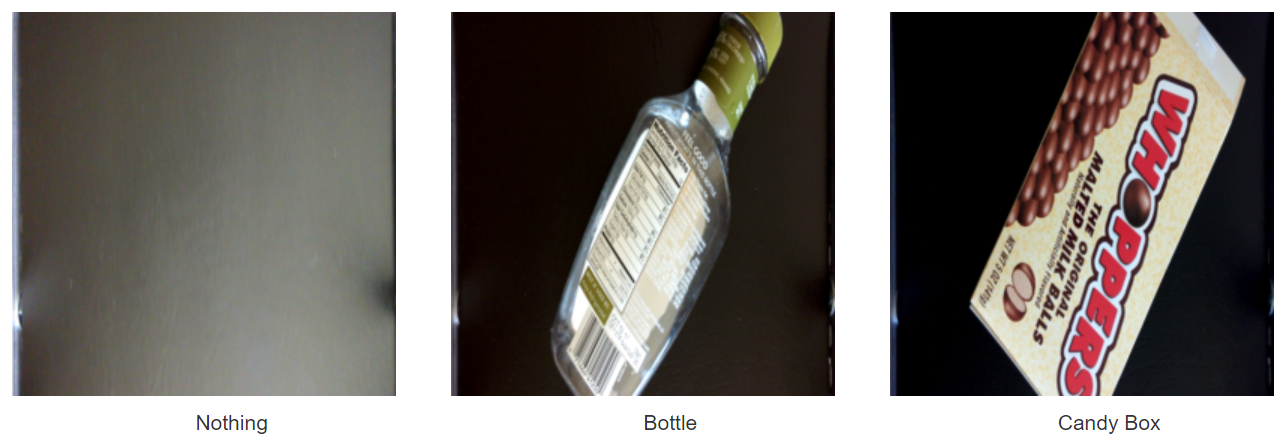
\includegraphics[width=\linewidth]{p_dataset.png}
      \caption{Supplied dataset}
      \label{fig:supplied_dataset}
\end{figure}

\subsection{Collected Dataset}

An additional dataset was collected using the built-in camera on a MacBook. To facilitate the capture process, a python script using the open-cv package was used. The PNG images were stored using a 256x256 pixel resolution following the folder structure used in DIGITS as the labels. 
The images were separated into three different categories "cube", "beaglebone", and "nothing" the distribution of each category is shown in Figure \ref{fig:categories}.
\begin{figure}[thpb]
      \centering
      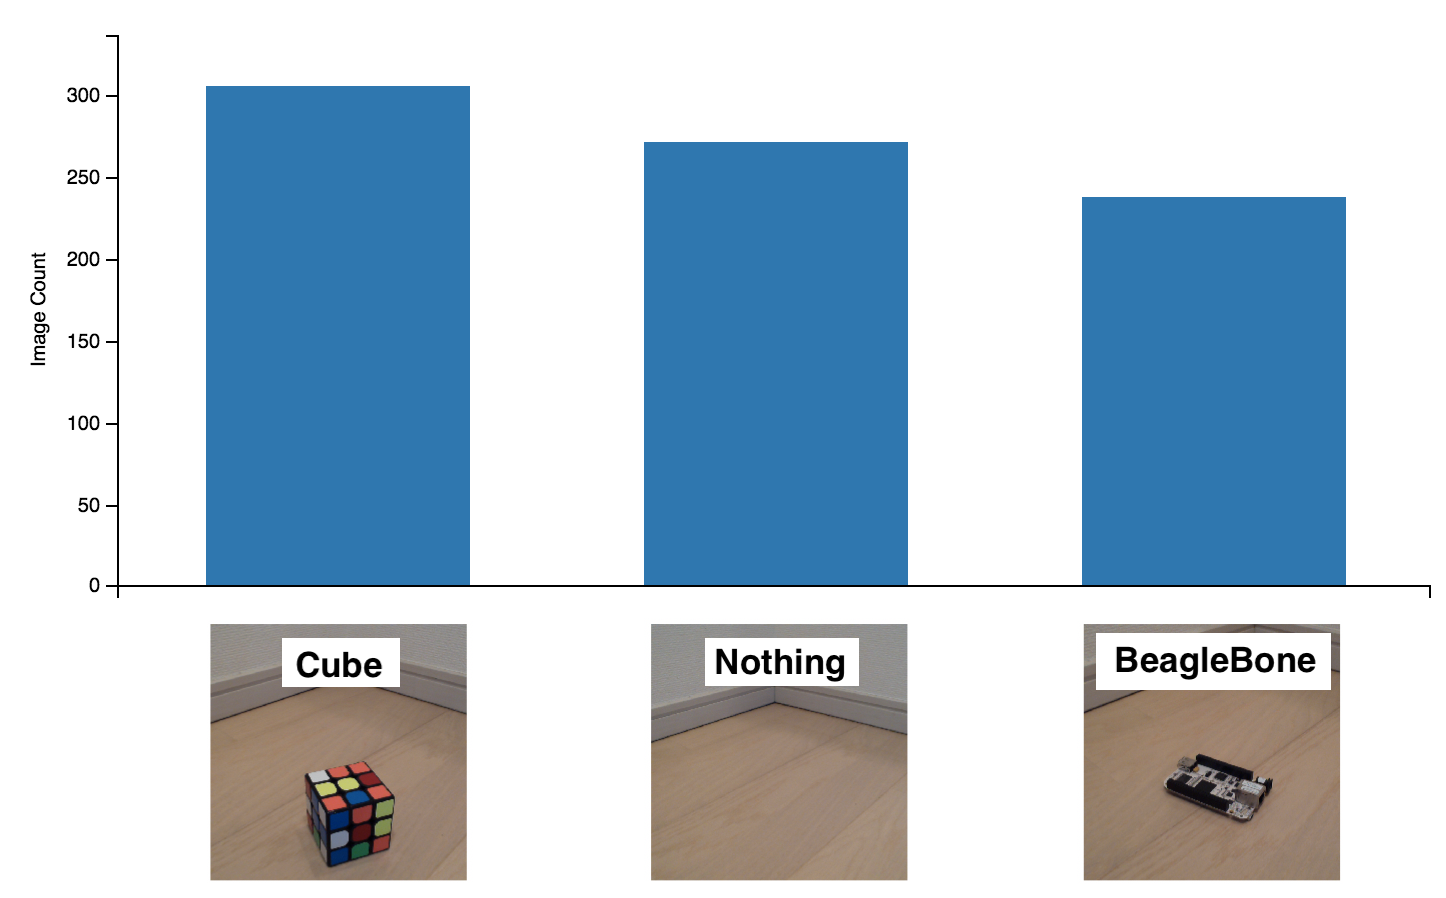
\includegraphics[width=\linewidth]{o_dataset_categories.png}
      \caption{Collected Dataset Categories}
      \label{fig:categories}
\end{figure}

A total of 1161 images was collected and separated into three groups: 70\% for training, 20\% for validation, and 10\% for testing. For simplicity, the objects were placed on the floor with a neutral background. Sample images can be seen on the Figure \ref{fig:collected_sample}.
\begin{figure}[thpb]
      \centering
      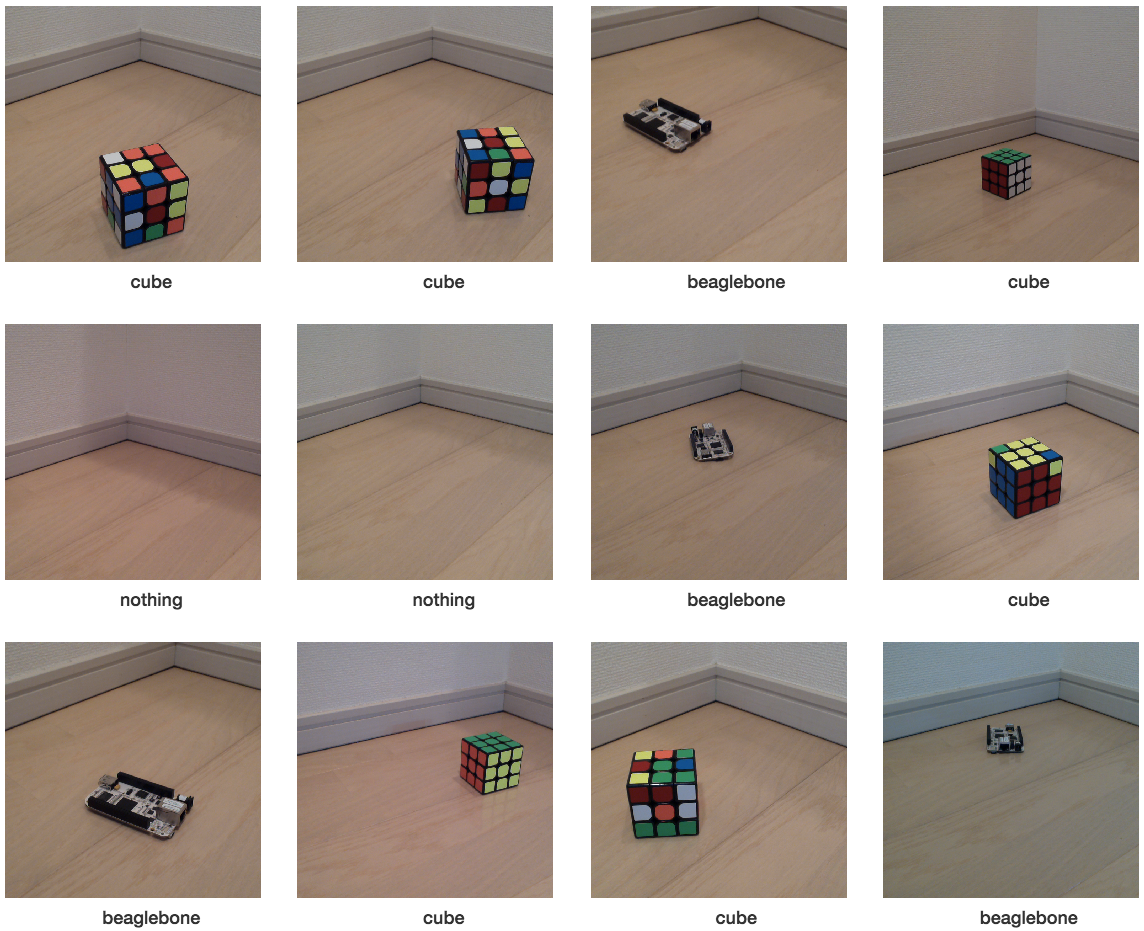
\includegraphics[width=\linewidth]{o_dataset_sample.png}
      \caption{Collected Dataset Sample}
      \label{fig:collected_sample}
\end{figure}



\section{Results}

\subsection{Supplied Dataset}

Figure \ref{fig:learning_curves} shows the learning curves obtained for the supplied dataset. It is possible to see that both models achieved scores close to 100\% for the validation set.
Using the 'evaluation' command, provided by Udacity, it was observed that both models achieved the same accuracy of 75.41\% using the test images. Training time for AlexNet was under 4 minutes while the training time for GoogLeNet three times longer. Inference time for the AlexNet was always bellow 5ms, while inference time for GoogLeNet was slightly above 5ms most of the time. 

\begin{figure}[thpb]
      \centering
      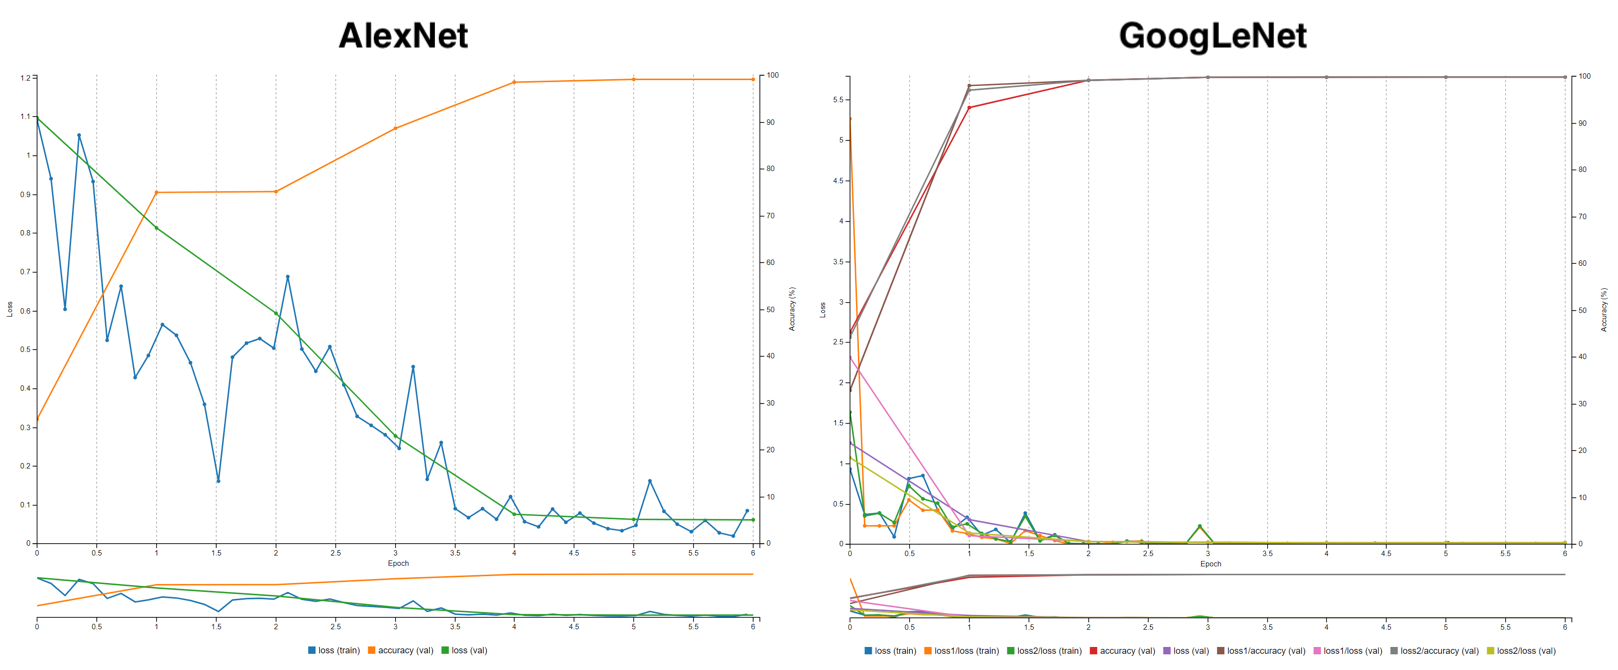
\includegraphics[width=\linewidth]{p_learning_curves.png}
      \caption{Learning curves on the Supplied dataset}
      \label{fig:learning_curves}
\end{figure}

\subsection{Collected Dataset}

In both cases, GoogLeNet and AlexNet, the models achieved accuracy above 95\% for the validation set and the test set. 
The test set was composed of 77 images. Figure \ref{fig:accuracy_comparisson} shows the confusion matrix for each model where only one image was misclassified.

\begin{figure}[thpb]
      \centering
      \subfloat[GoogLeNet]{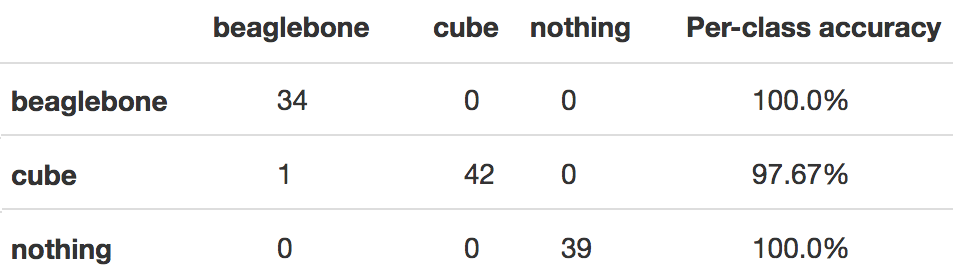
\includegraphics[width=0.9\linewidth]{o_gln_accuracy.png}\label{fig:acc-gln}}
      \vfill
      \subfloat[AlexNet]{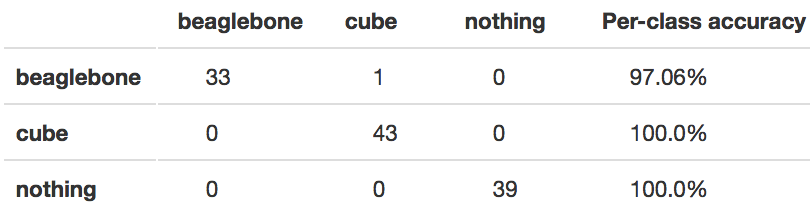
\includegraphics[width=0.9\linewidth]{o_aln2_accuracy.png}\label{fig:acc-aln}}
%      \vspace{0.5cm}
%      \includegraphics[width=\linewidth]{loss-accuracy-curve-legend}
      \caption{Accuracy comparison}
      \label{fig:accuracy_comparisson}
\end{figure}


When using the AlexNet, the original learning rate was decreasing fast and the best score for the validation set was under 85\%. Figure \ref{fig:learning_rate_comparisson} shows that after training the network with a higher learning rate, results of approximately 95\% accuracy for the validation set was achieved.

\begin{figure}[thpb]
      \centering
      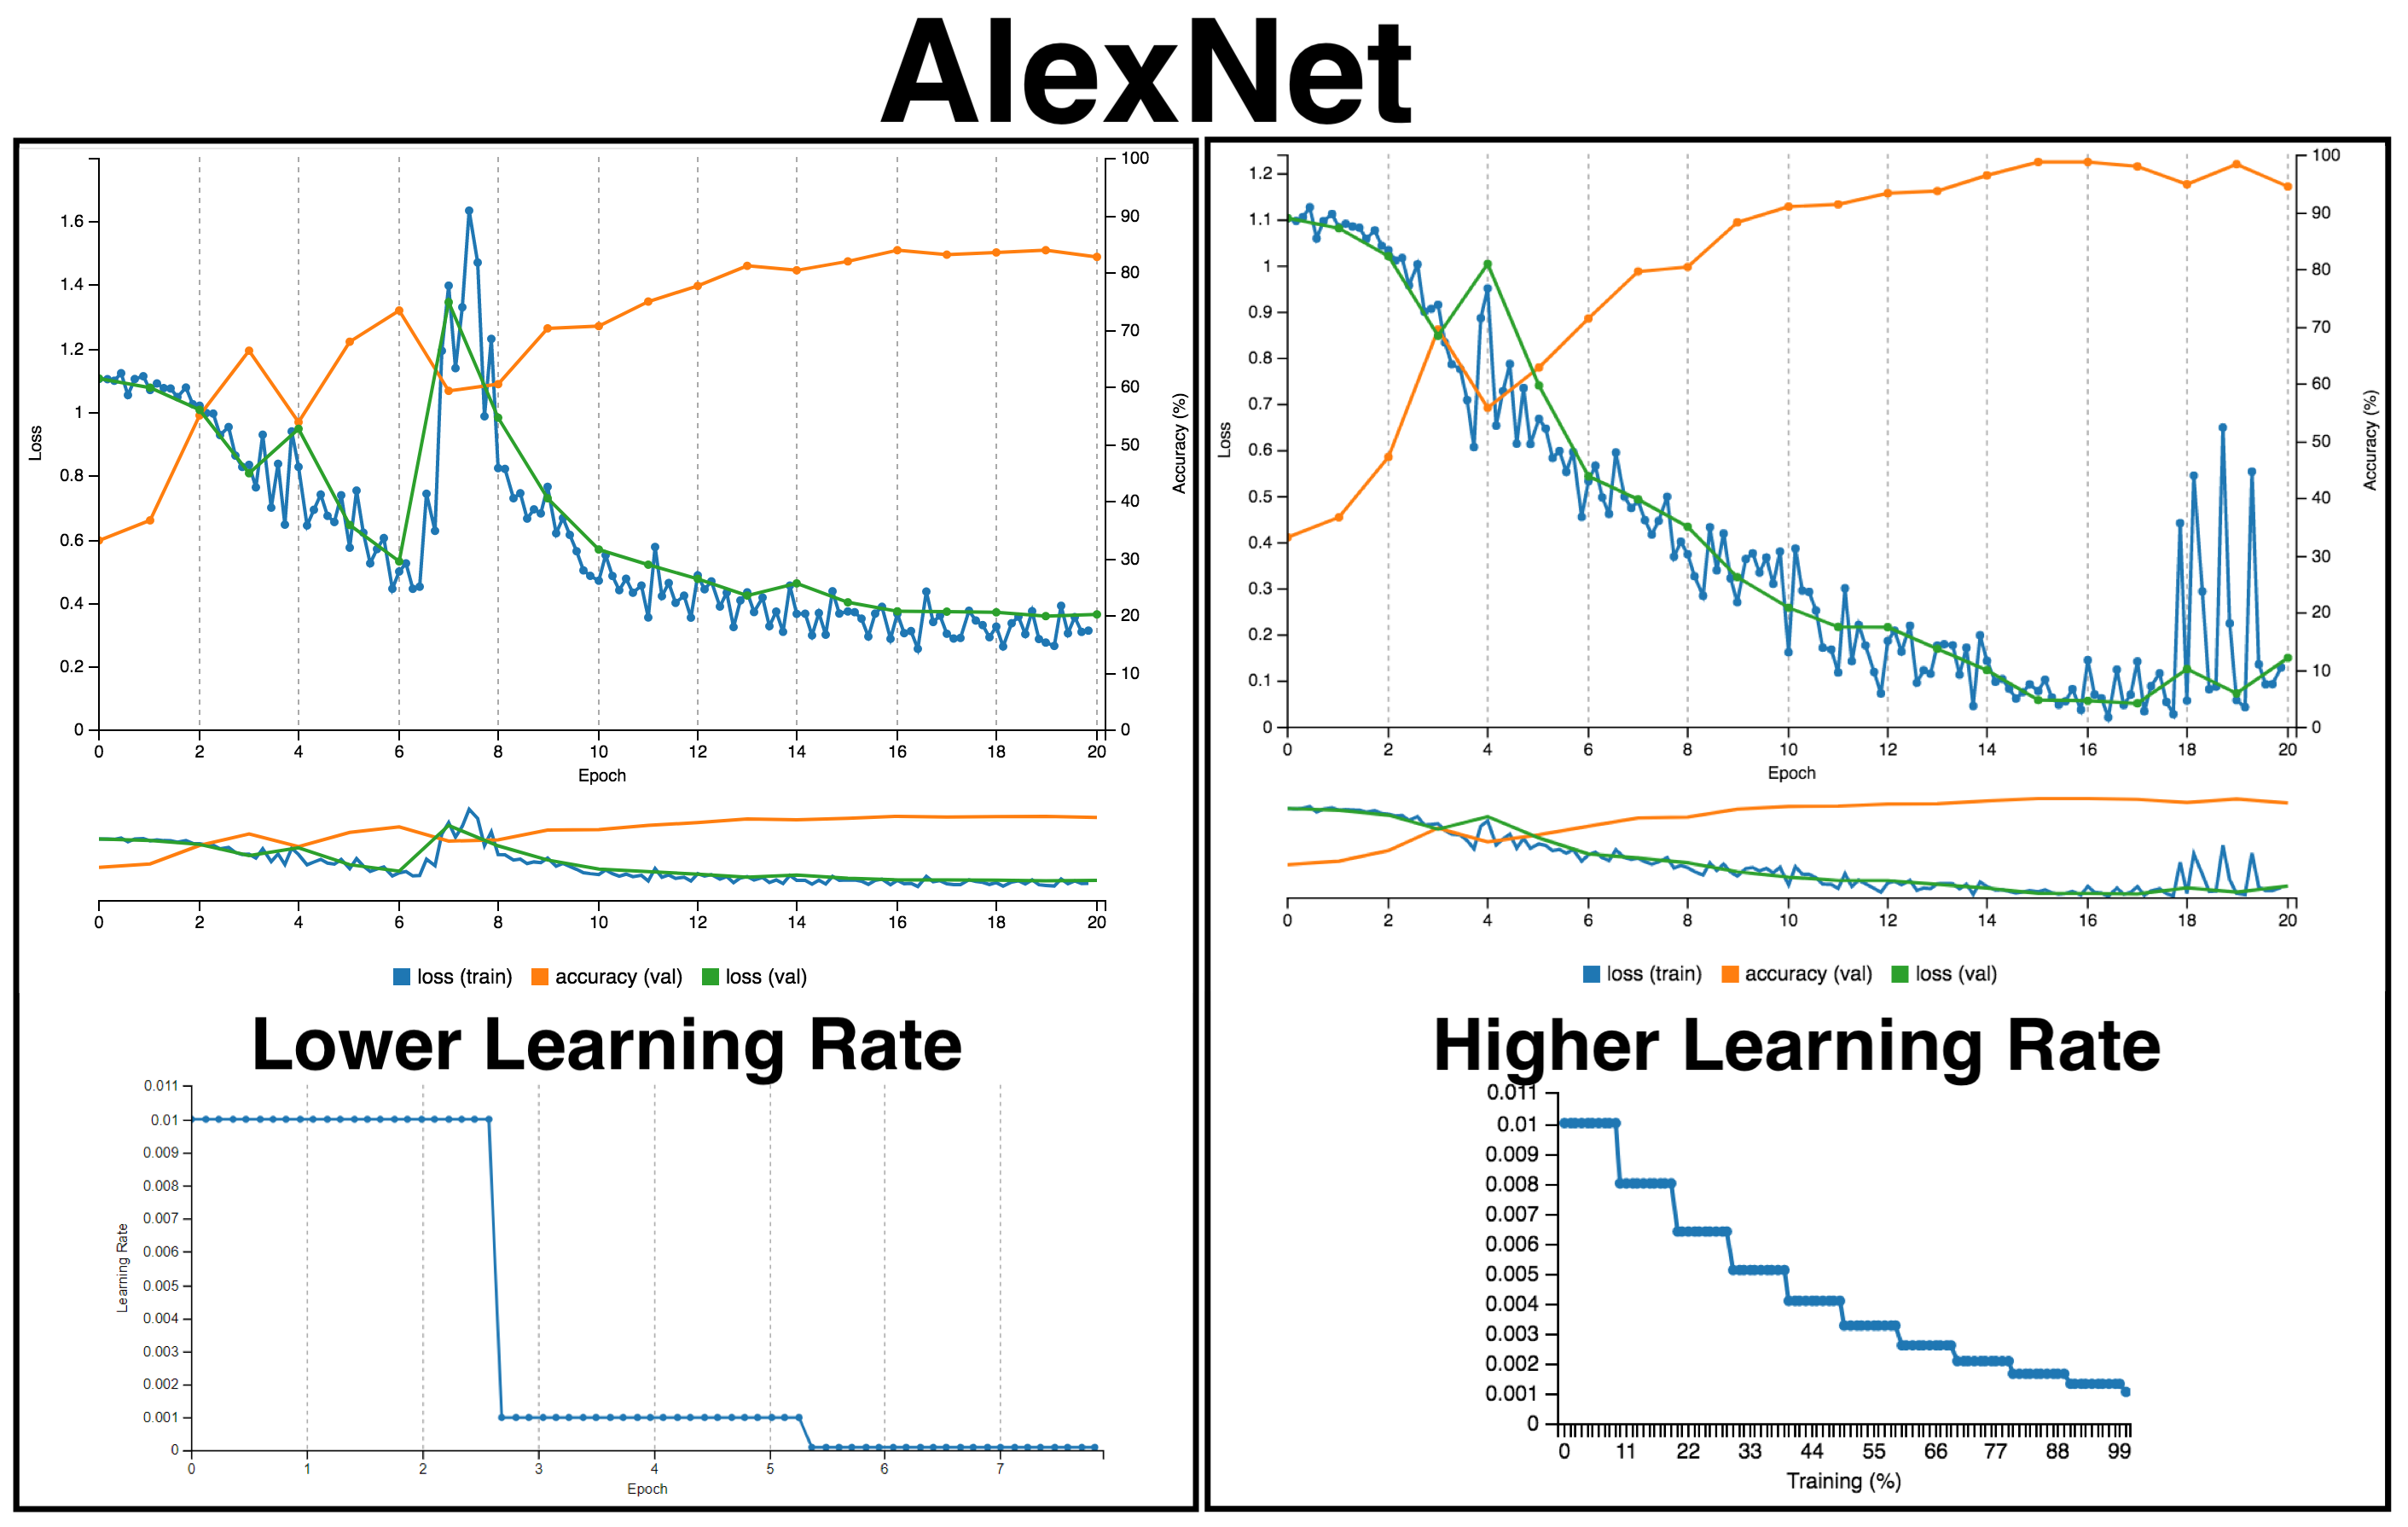
\includegraphics[width=\linewidth]{o_aln_training_comparisson.png}
      \caption{Learning Rate Comparison}
      \label{fig:learning_rate_comparisson}
\end{figure}


\section{Discussion} 
\label{discussion}
\subsection{Supplied Dataset}

The provided dataset was very helpful to quickly start learning how to use the DIGITS workspace to train Neural Networks for image recognition.
The results obtained using GoogLeNet and AlexNet were very similar. It is worth noting that the accuracy achieved in the test set (75\%) is much lower to the accuracy achieved during training for the validation set (higher than 90\%). It indicates that the trained model is failing to generalize or the model is overfitted.
Considering the lower training time and the slightly faster inference time, one could choose to use AlexNet. Nevertheless, in the provided application, battery consumption is not a concern. Therefore, GoggLeNet can be selected and after additional training with a more complete dataset, better results could potentially be achieved. 

\subsection{Collected Dataset}

Both networks performed very well on the validation and on the test images. Apparently, it is a very good result, but on the other hand, it can also indicate that the model is overfitted, especially considering that the dataset used is very small.
 
Further inspecting the image that was misclassified in the GoogLeNet network, it was possible to verify the pixels from the background of the image were responsible for the activation of the network. Figure \ref{fig:activation} shows an example of the activation in one convolutional layer. This evidence corroborates with the assumption that the network is overfitted. 
\begin{figure}[thpb]
      \centering
      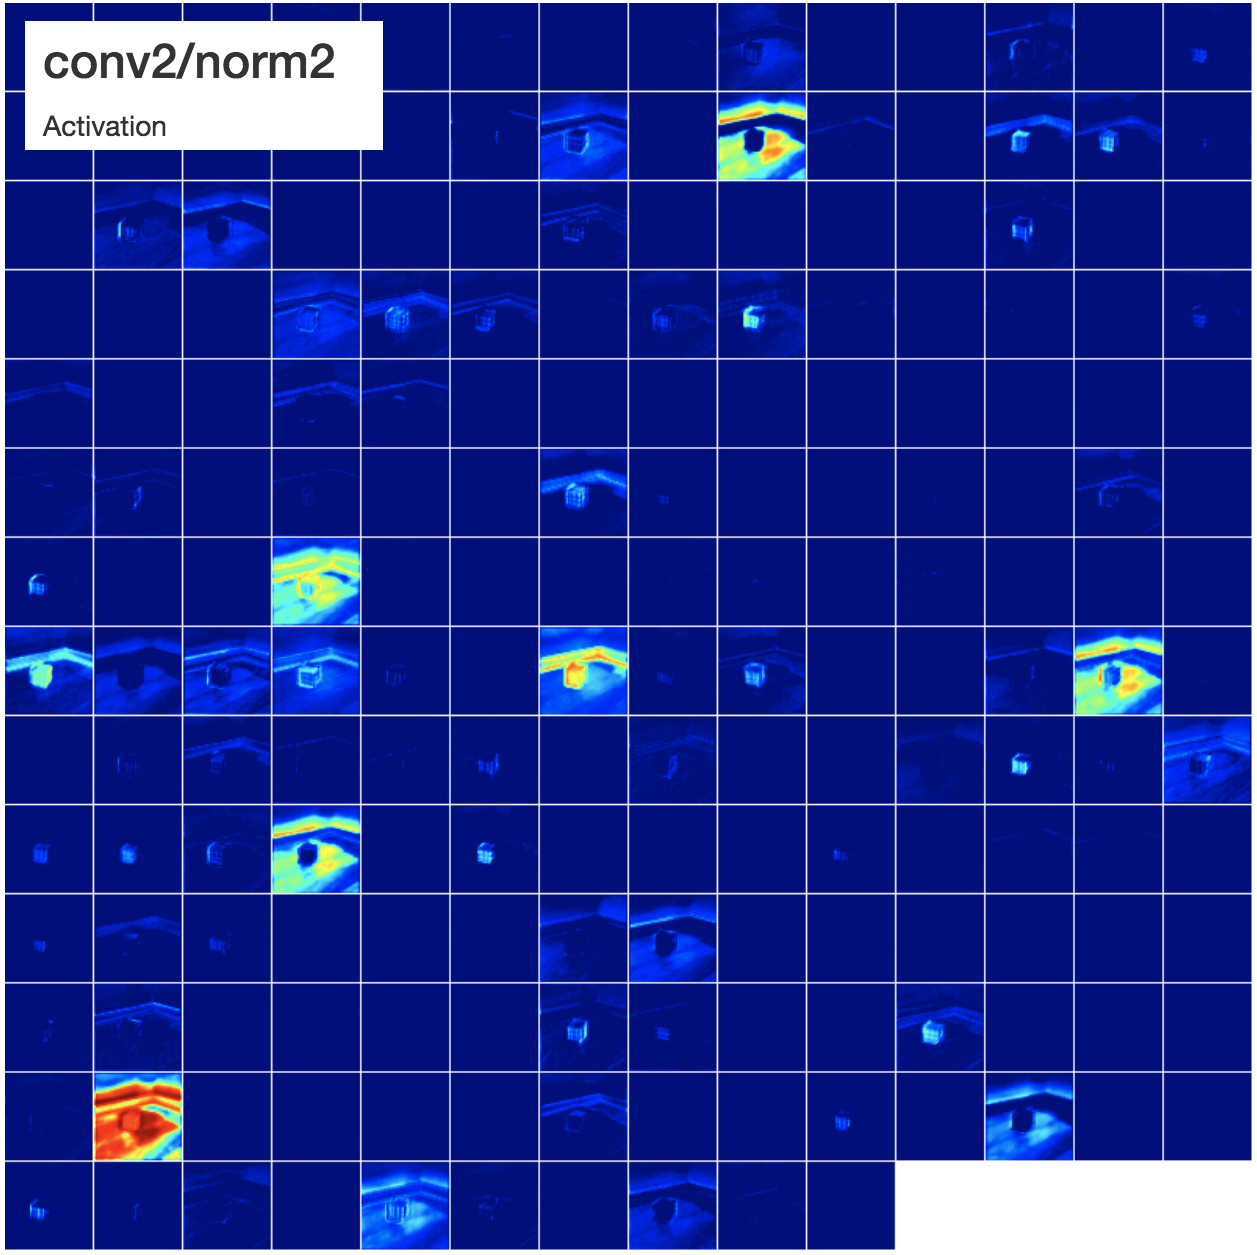
\includegraphics[width=\linewidth]{o_err2.png}
      \caption{Convolution Layer Activation}
      \label{fig:activation}
\end{figure}

When training the GoogLeNet network, high accuracy on the validation set was achieved very early. Selecting the model achieved on the epoch number 4 would significantly decrease the learning time while preventing the network to overtrain.

Given that all images provided in this dataset were captured with a very similar background, it is plausible to assume that the accuracy is expected to decrease significantly when the objects are placed in different environments. 

For the collected dataset the inference time was not measured since the evaluation was performed in the DIGITS workspace.


\section{Conclusion}

Despite achieving a high accuracy for the test dataset, the current models may not perform well for the target application of locating objects anywhere in the house autonomously. It is far from a commercially viable product. Nevertheless, it achieved the main learning goals and has laid the foundation for future work. The project was great to understand the core challenges of training a Neural Network, especially the notion that accuracy is not the only important parameter to be considered. Inference time and model complexity are equally important, especially for robotic applications. It was also important to get a sense of how much the quality of the dataset has a strong influence on the results.


\section{Future work}

The first activity to be done in the future is to deploy both models in hardware with lower performance and compare the inference performance. Later, the models can be further improved by collecting more data and enhancing the training dataset with several augmentation techniques. 
Finally, the goal is to include not only the classification step but also improve the perception pipeline to execute a complete segmentation task.


\bibliography{bib}
\bibliographystyle{ieeetr}

\end{document}

